\section{Extrapolations to higher luminosity}
\label{sec:extrapolations}

Future runs of the LHC expect to deliver significantly higher instantaneous luminosity than current operations. To cope with these harsher data-taking conditions, upgrades to the muon spectrometer are planned. In Long Shutdown 2 (LS2), which is scheduled to start in 2018, the current endcap small wheels will be replaced by the New Small Wheels (NSW) equipped with small Thin Gap Chambers and MicroMegas detectors. In Long Shutdown 3, which is scheduled to start near 2022, the MDT electronics are being considered for replacement, and additional coverage for the barrel muon trigger system is under consideration.

A crucial ingredient in the planning of these upgrades is the hit rate of incident particles the detectors are expected to receive. This section presents an expected rate in the hottest regions of the MS as extrapolated from data-taking in 2015. This extrapolation does not address potential changes in the shielding of the MS or the beampipe, which can have a large effect and must be characterized with simulation. The hottest regions of the MS in 2015 data are the innermost regions of the endcap inner small wheel (CSC L, CSC S, MDT EIL1, MDT EIS1) and endcap middle big wheel (EML1, EMS1).

The prediction is performed by considering the hit rates in 2015 data-taking as a function of the instantaneous luminosity, fitting the linear dependence, and extrapolating to higher luminosity. These rates are shown in Section~\ref{sec:hitrates} with linear fits overlaid.

The parameters of the linear fit depend on the number of filled bunches in the LHC, as expected. The maximum number of filled bunches in 2015 is 2232 bunches, whereas Run 3 of the LHC is expected to fill at most 2808 bunches, and the HL-LHC is expected to fill at most 3564 bunches. To extrapolate to more filled bunches, the fitted slopes are considered for 2015 runs with as few as 447 filled bunches and as many as 2232 bunches, and the dependency is extracted by fitting this spectrum to a first-order inverse power law, as shown in Figure~\ref{fig:extrapolations-slope-vs-bunches-raw} with vertical lines at 2808 and 3564 filled bunches. The fitted slopes are the same as reported in Figures~\ref{fig:hitrates-vs-lumi-csc-raw}, \ref{fig:hitrates-vs-lumi-mdt-ei1-raw}, and \ref{fig:hitrates-vs-lumi-mdt-em1-raw}.

\begin{figure}
  \begin{center}
    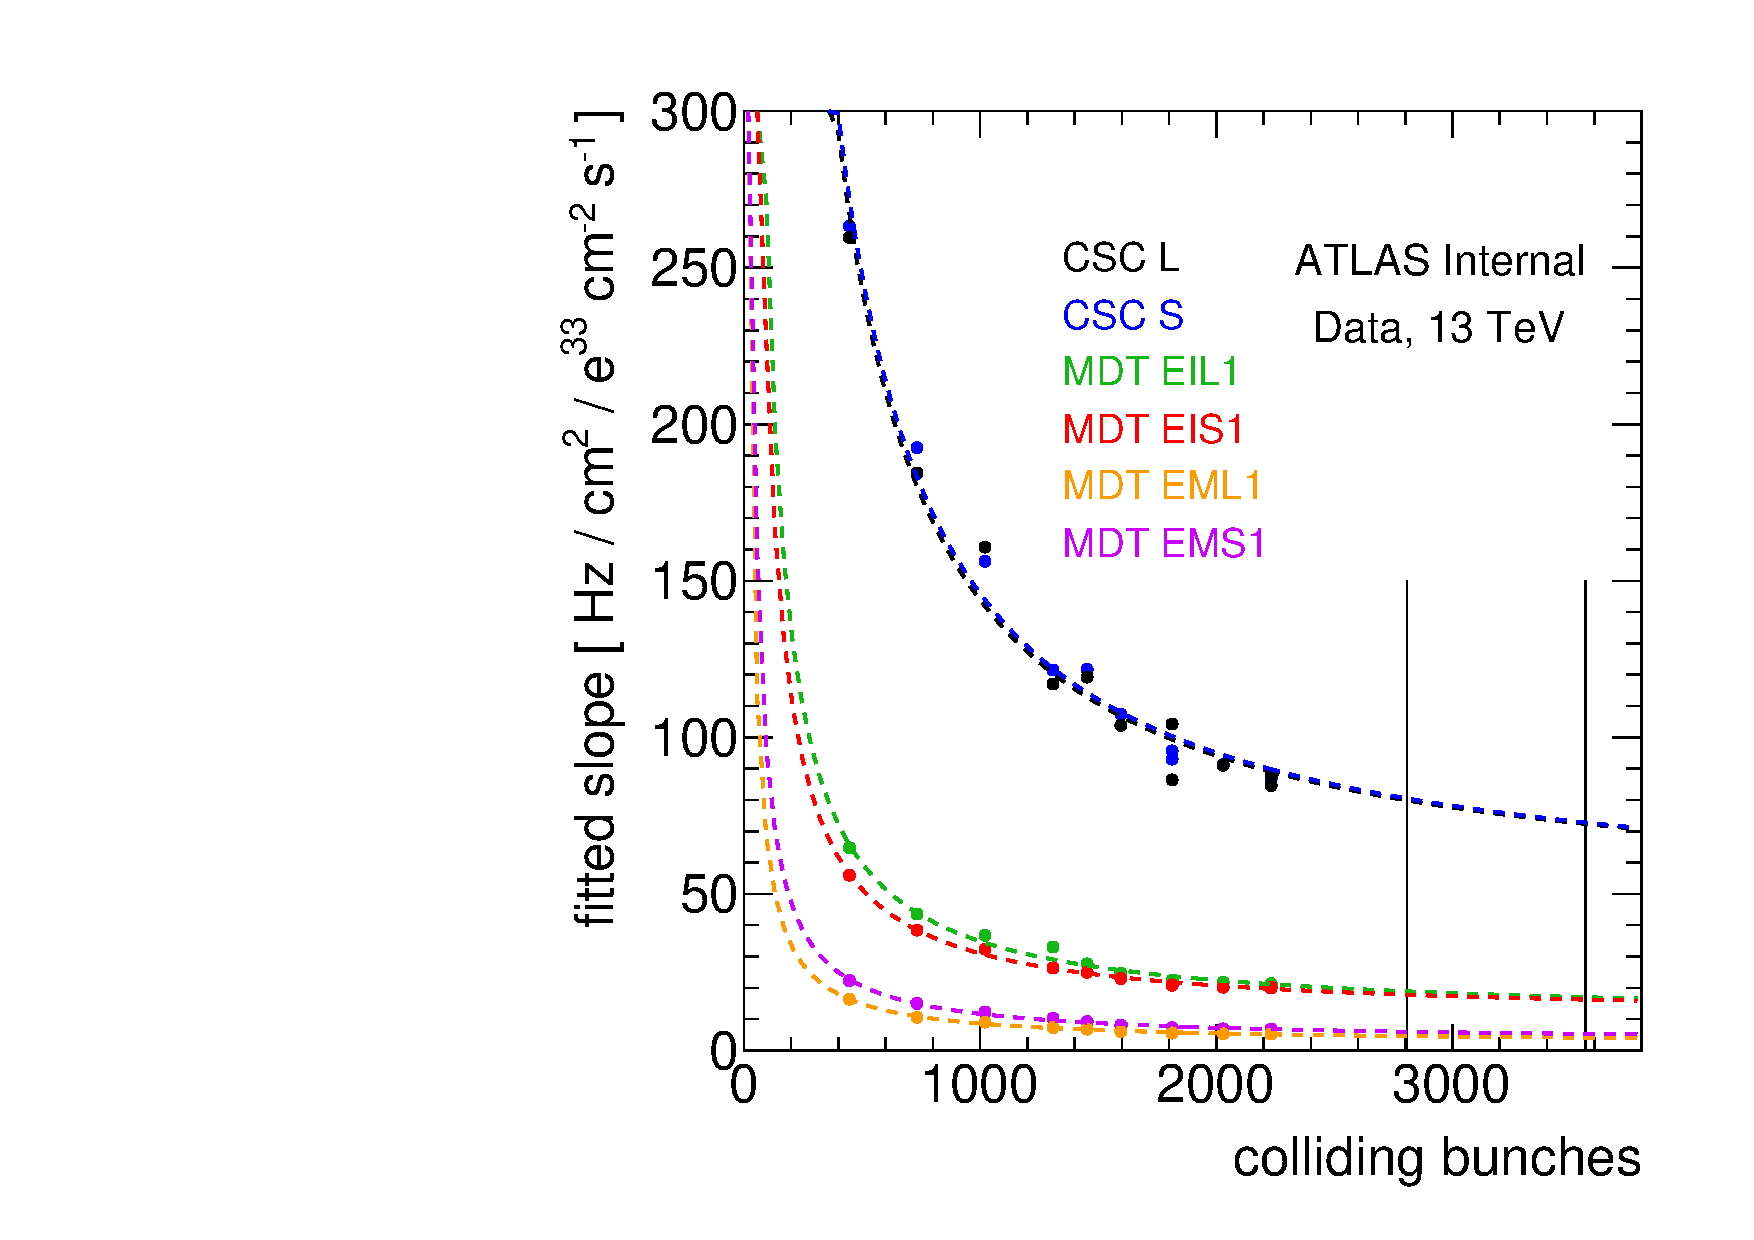
\includegraphics[width=0.45\textwidth]{./figures/slope_vs_bunches_raw_lin.pdf}
    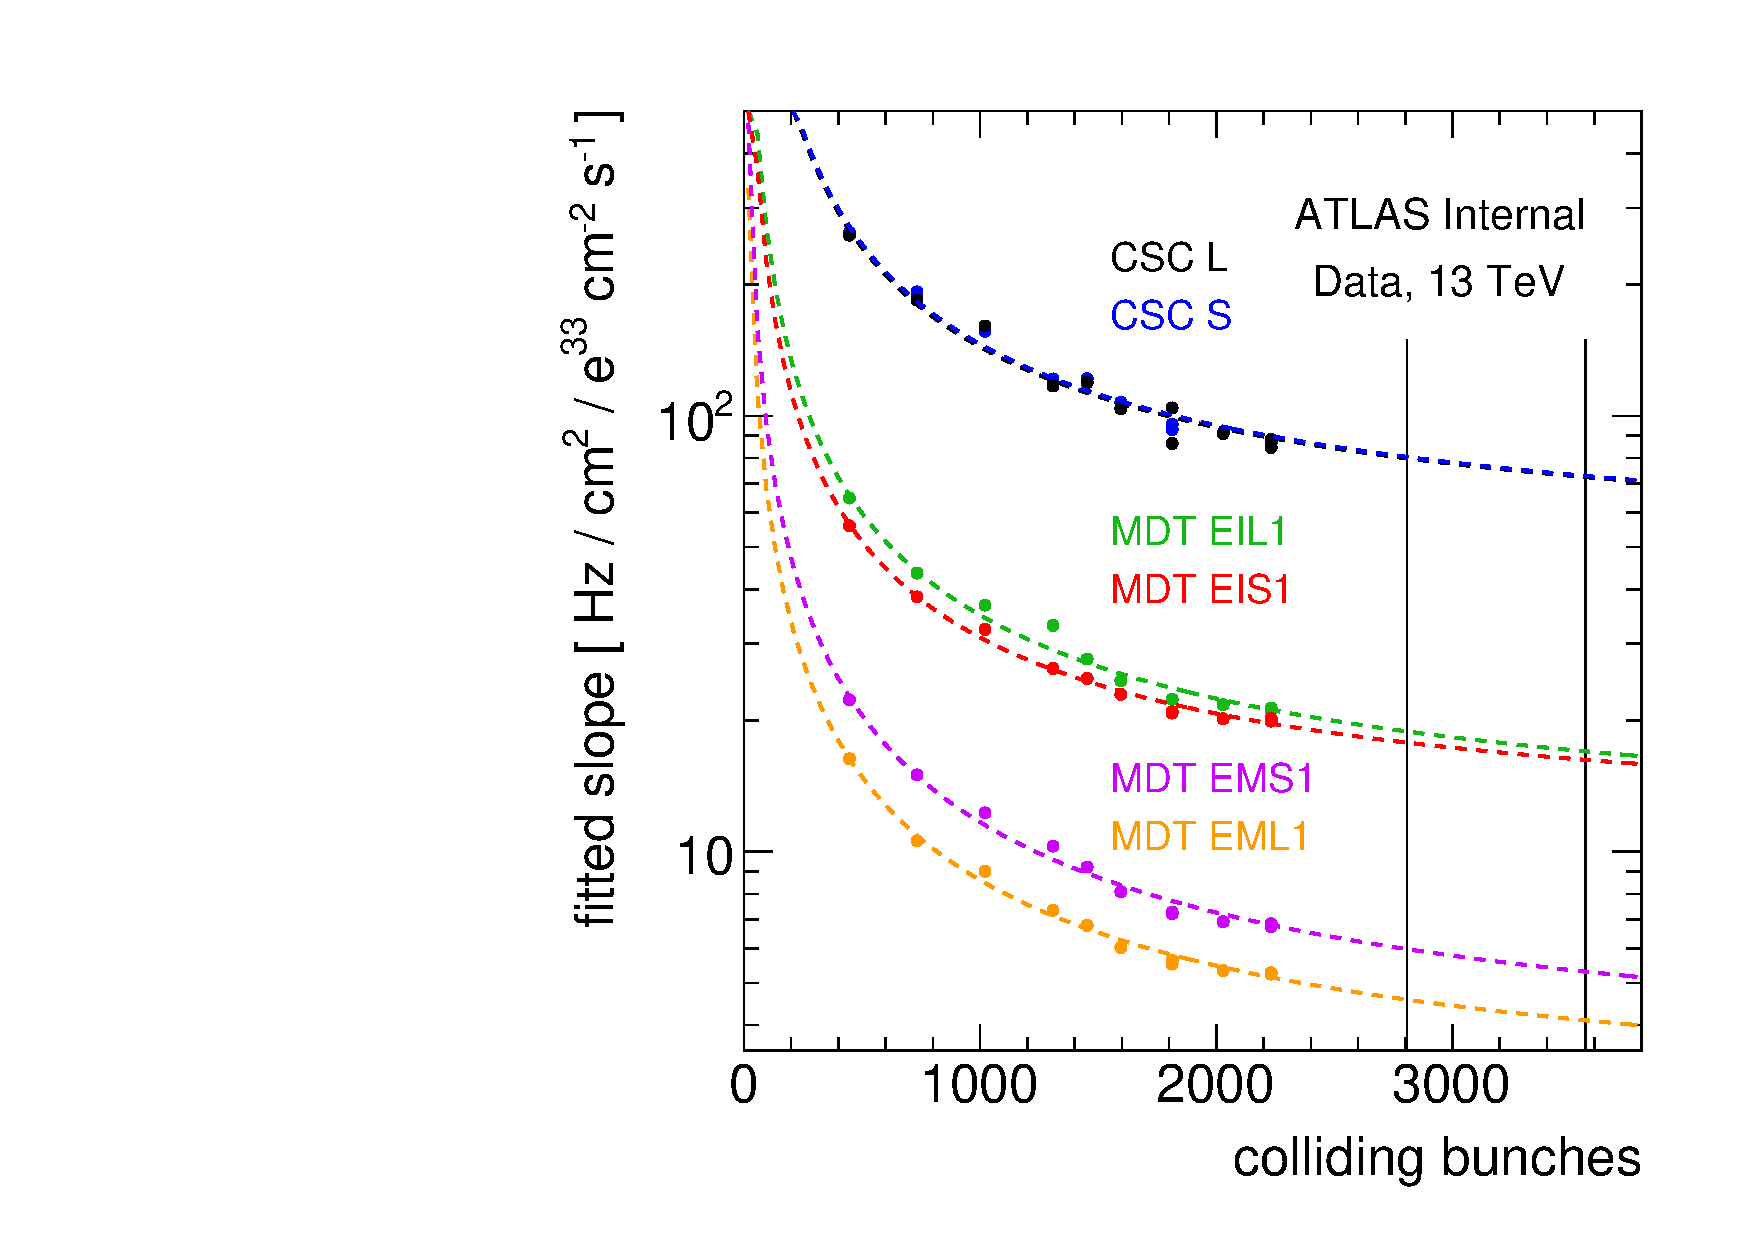
\includegraphics[width=0.45\textwidth]{./figures/slope_vs_bunches_raw_log.pdf}
    \caption{The fitted slope as a function of the number of colliding bunches for various runs in the hottest MDT and CSC chambers, shown with linear (left) and logarithmic (right) scale. The spectra are fitted to $A + B/x$, where $x$ is the number of bunches.}
    \label{fig:extrapolations-slope-vs-bunches-raw}
  \end{center}
\end{figure}

This fit gives parameters for the linear dependence of hit rate on instantaneous luminosity at more filled bunches than was reached in 2015. The projected average hit rates for the hottest chambers of the MS are shown in Figure~\ref{fig:extrapolations-hitrates-raw}. The large (L) and small (S) sectors of a give detector region have similar projected hit rates.

\begin{figure}
  \begin{center}
    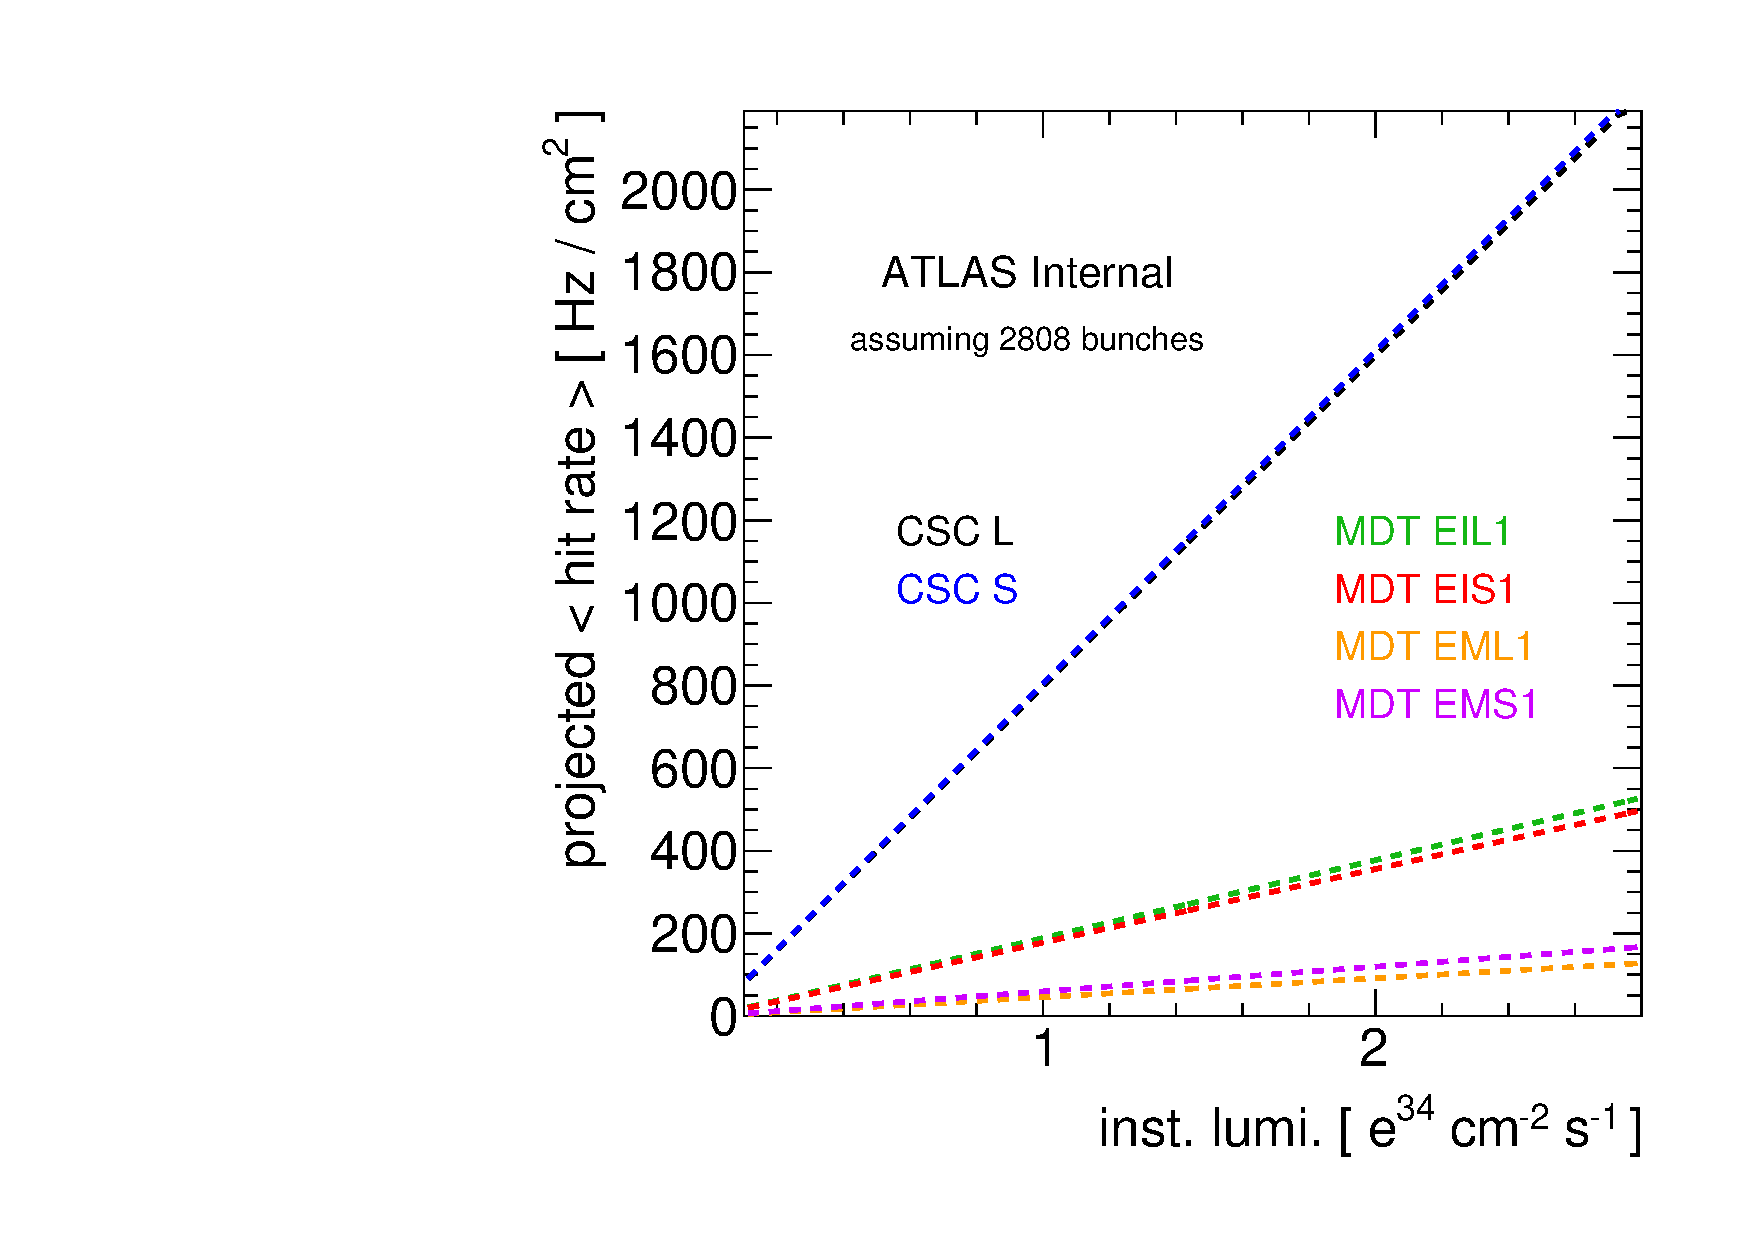
\includegraphics[width=0.45\textwidth]{./figures/extrapolate_vs_lumi_raw_2808.pdf}
    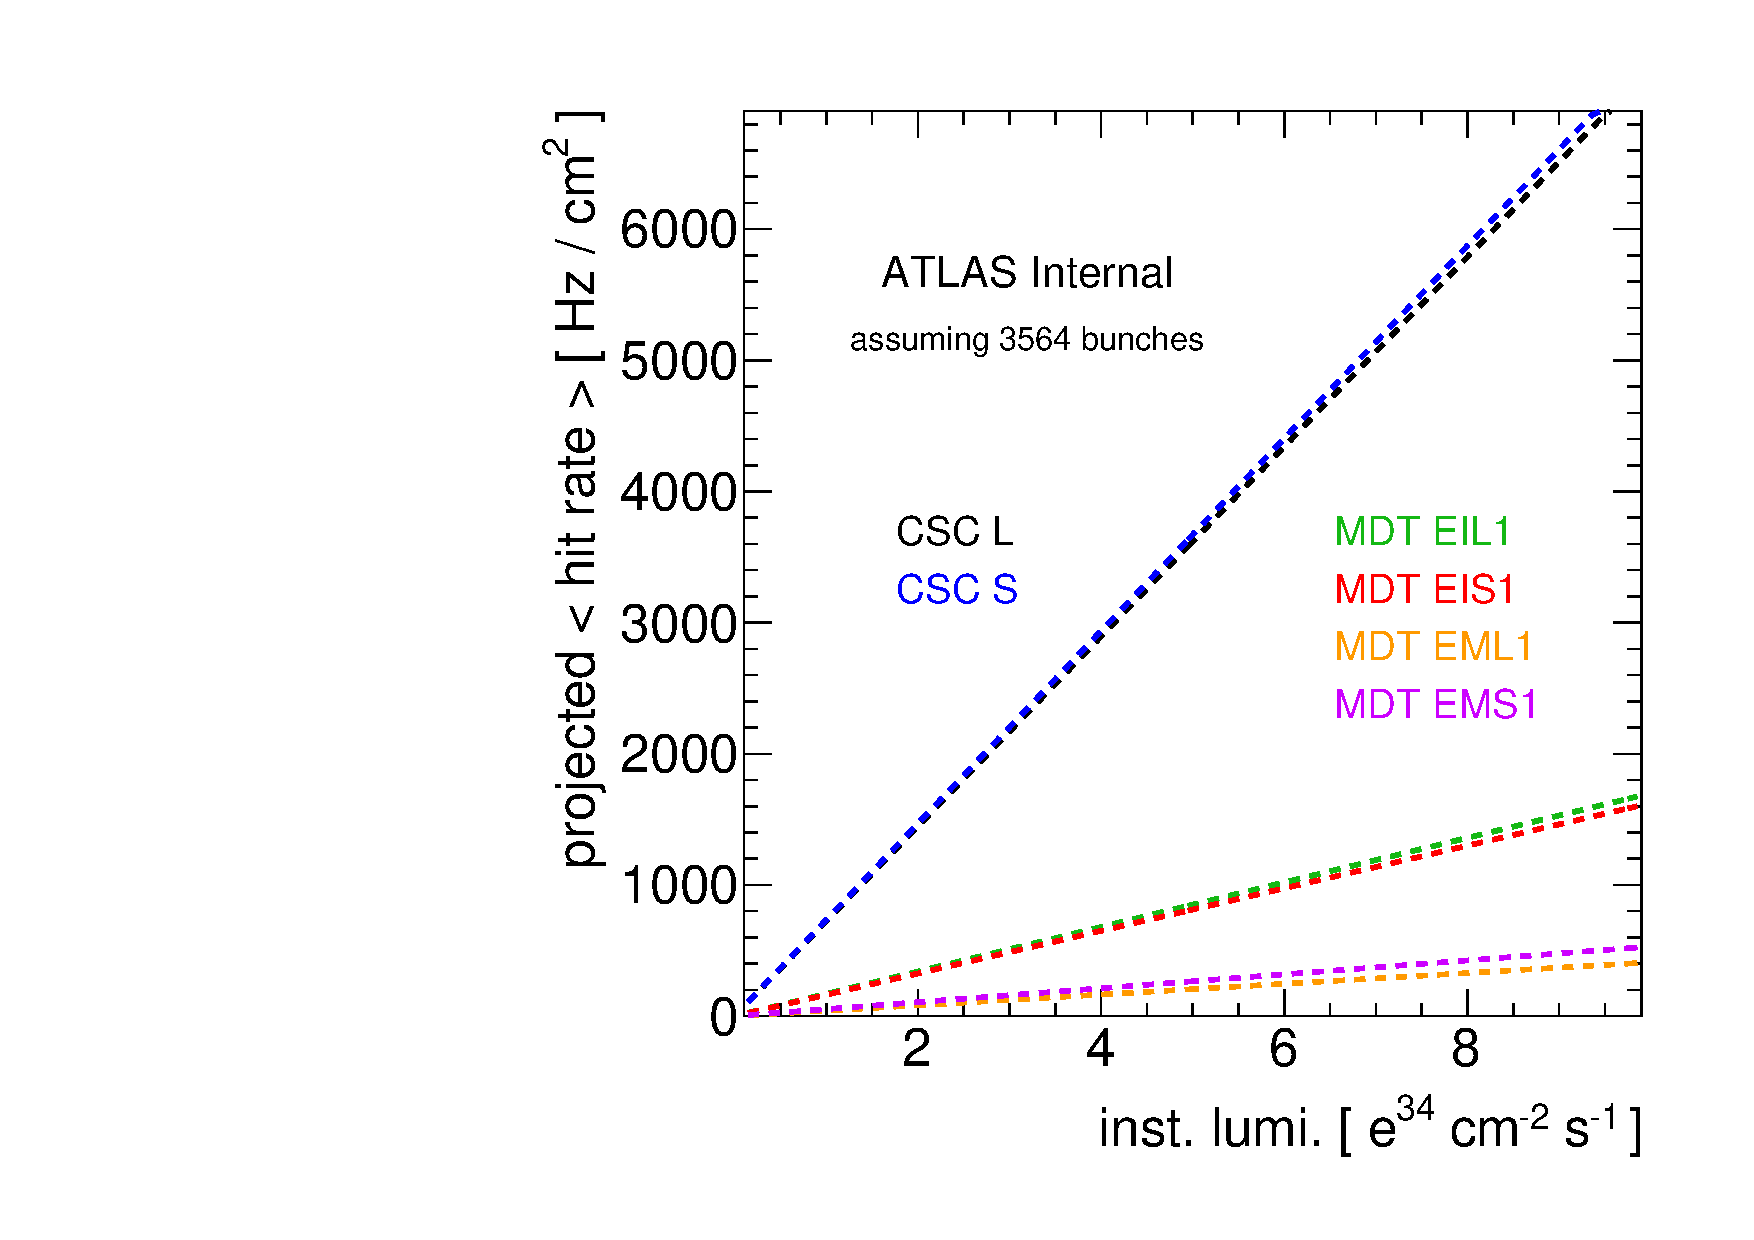
\includegraphics[width=0.45\textwidth]{./figures/extrapolate_vs_lumi_raw_3564.pdf}
    \caption{Projected average hit rates in the MS as a function of instantaneous luminosity, assuming 2808 (left) and 3564 (right) filled bunches in the LHC. The CSC and MDT EI regions are overlaid.}
    \label{fig:extrapolations-hitrates-raw}
  \end{center}
\end{figure}

The projected average hit rates at Run 3 and HL-LHC conditions are shown in Table~\ref{tab:extrapolations-hitrates-raw}. The instantaneous luminosity is assumed to be $2\times10^{34}$ in Run 3 and $7\times10^{34}$ at the HL-LHC. 

\begin{table}
  \begin{center}
    \renewcommand{\arraystretch}{1.4}
    \begin{tabular}{c|c|c}
      \multicolumn{1}{c}{} & \multicolumn{2}{c}{\rate} \\
      \hspace{0.6cm}Region\hspace{0.6cm} & \hspace{0.6cm}Run 3\hspace{0.6cm} & HL-LHC   \\
      \hline\hline
      CSC L        & 798.7     & 5065.2 \\
      CSC S        & 804.7     & 5095.2 \\
      \hline
      MDT EIL1     & 188.7     & 1189.4 \\
      MDT EIS1     & 177.9     & 1137.0 \\
      \hline
      MDT EML1     &  45.8     &  287.3 \\
      MDT EMS1     &  59.8     &  371.5 \\

      % adc
      % CSC L        & 697.0     & 4399.66 \\
      % CSC S        & 708.6     & 4479.66 \\
      % \hline
      % MDT EIL1     & 160.4     & 1007.13 \\
      % MDT EIS1     & 151.8     &  967.57 \\
      % \hline
      % MDT EML1     &  38.6     &  241.16 \\
      % MDT EMS1     &  50.1     &  308.94 \\

    \end{tabular}
    \caption{Projected average hit rates at Run 3 and HL-LHC conditions in the hottest regions of the MS. Run 3 conditions assume $\mathcal{L}=2\times10^{34}$ and 2808 filled bunches in the LHC. HL-LHC conditions assume $\mathcal{L}=7\times10^{34}$ and 3564 filled bunches.}
    \label{tab:extrapolations-hitrates-raw}
  \end{center}
\end{table}

The CSC hit rate in 2015 data-taking closest to the beampipe is 1.94 (2.23) times larger than the average hit rate of the large (small) chambers, as discussed in Section~\ref{sec:hitrates}. This implies the hottest region of the NSW will have a hit rate of between 9827 and 11362 $\text{Hz} / \text{cm}^2$, depending on the number of filled bunches in the LHC, and assuming no changes to the shielding of the MS or the beampipe. These extrapolations include contributions from electronic noise in the CSCs and MDTs, which are expected to inflate the rates by 10-20\%.


